\chapter{What is origami?}
Origami is the name of an ancient Asian art of folding various figures and shapes from a sheet of paper.

"Whether it is called `zhe zhi,' as it is by Mandarin-speaking Chinese, or `chip chee,' as Chinese who use the Cantonese dialect call it, or by the Japanese name `origami,' it is generally agreed that the art of paperfolding originated in China perhaps before the 6th century." \cite[p. 123]{temko}

The traditional Japan origami focuses mainly on animal figures and flowers. You could know the most famous origami animal - the crane. It is considered as a sample of the traditional technique.

In recent times, hundreds of other origami models can be found, including boxes, decorations and ornaments, envelopes, abstract things and much more. \cite{lang}

\begin{figure}
	\centering
	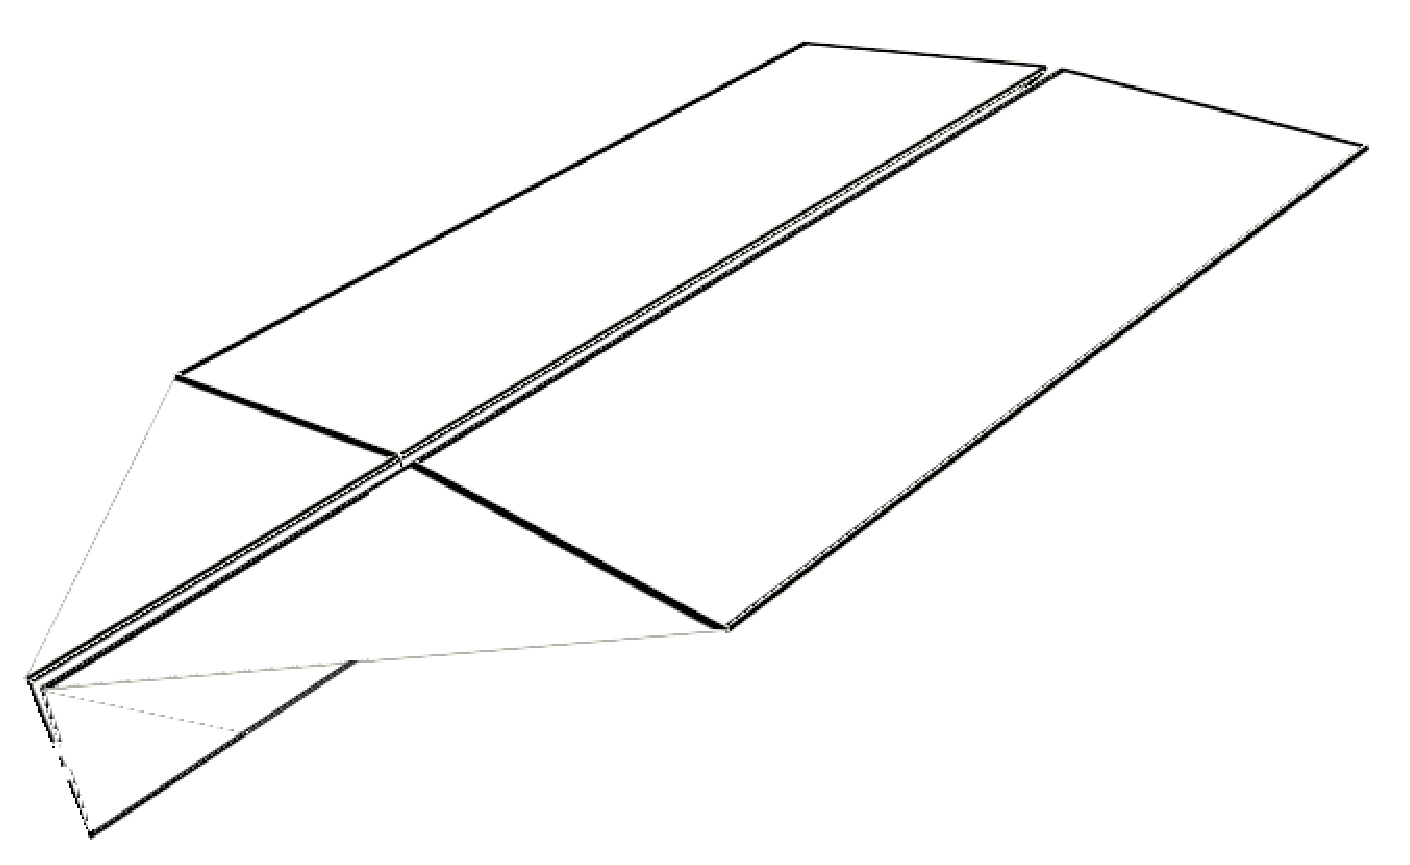
\includegraphics[width=15cm]{images/preview01}
	\caption{Origami model of a paper plane}
\end{figure}

\section{The rules of traditional origami}
There aren't much constraints in the traditional origami. Everyone can fold whatever his fantasy invents, but to call the model a traditional origami, there are these rules: \cite{pen}
\begin{itemize}
\item To begin with a single square sheet of paper.
\item Not to tear or cut the sheet of paper.
\item Not to use glue.
\end{itemize}
And that's it. No more constraints on what can be done. This is also the set of rules Origamist tries to hold (in fact, it allows non-square papers).

\section{Other kinds of origami}
Besides the traditional origami, there are several other types, differing in what is allowed or disallowed. Here is a short list of some other techniques:
\begin{itemize}
\item \emph{Modular origami}, which allows to use and combine multiple sheets of paper. \cite{fuse}
\item \emph{Action origami}, which creates figures whose parts are moveable, so they can be used as toys. \cite{lang2}
\item \emph{Pureland origami}, which only allows one fold to be done at once, and thus disallows folds like reverse folds or rabbit folds. This type of origami is suitable for beginners, children and disabled people. \cite{smith}
\item \emph{Kirigami}, which allows cutting the paper and using glue. Kirigami is mostly used to make decorations. \cite{temko2}.
\item \emph{Technical origami}, which develops the models based on computer-generated crease patterns (more on crease patterns can be found in \ref{sec:creasePatterns}). \cite{mobilereference}.
\item \emph{Mathematical origami}, which is just abstract and is used for some mathematical and algorithmic proofs.
\item \emph{Rigid origami}, which is a subset of mathematical origami and tries to find answers to the question "If we replaced paper with sheet metal and had hinges in place of the crease lines, could we still fold the model?" \cite{mobilereference}.
\end{itemize}

\section{Basic folds}
\label{sec:basicFolds}
In this section, some basic fold types will be described, as will be the common marks for them. Sample images are taken from \cite{folds}, the descriptions of the steps are inspired by \cite{lang}.

\begin{savenotes}
\begin{longtable}{lp{5.5cm}}
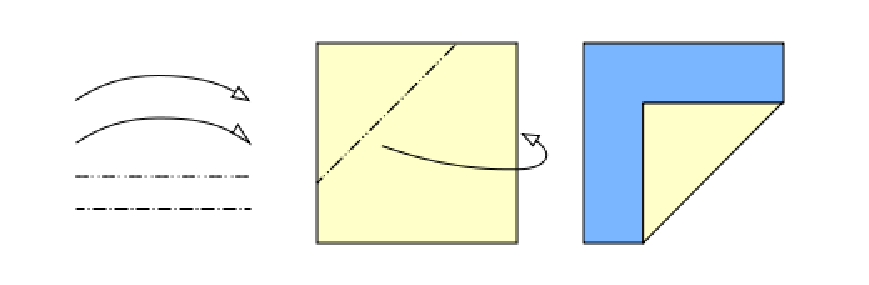
\includegraphics[width=7.5cm]{images/folds_mountain} & \emph{Mountain fold}. This is a simple fold which bends the paper in the direction `from the viewpoint'. An arbitrary angle can be specified for this type of fold.\\
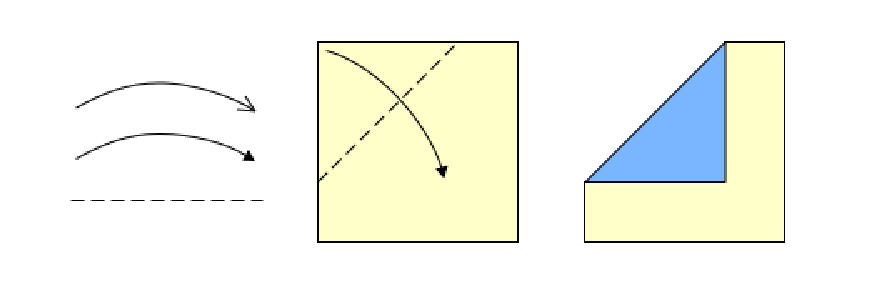
\includegraphics[width=7.5cm]{images/folds_valley} & \emph{Valley fold}. This is a simple fold which bends the paper in the direction `towards the viewpoint'. An arbitrary angle can be specified for this type of fold.\\
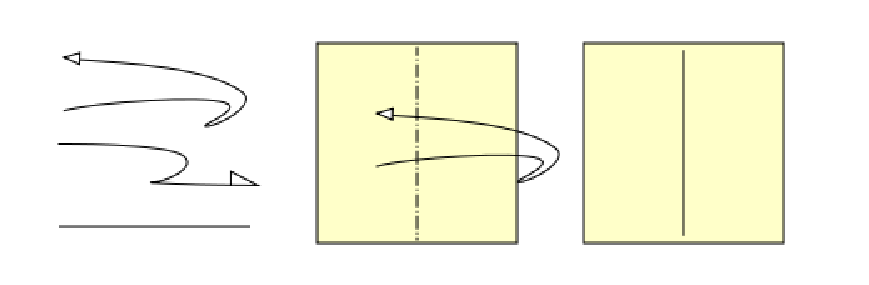
\includegraphics[width=7.5cm]{images/folds_fold_unfold_mountain} & \emph{Mountain fold and unfold}. This fold just makes a mountain crease on the paper. After doing it, the paper has the same geometry as before, but the crease has required moving the paper. This is mainly used for creating reference creases.\\
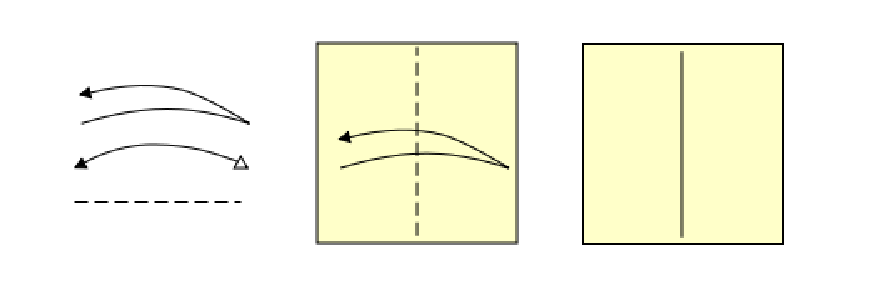
\includegraphics[width=7.5cm]{images/folds_fold_unfold_valley} & \emph{Valley fold and unfold}. This fold just makes a valley crease on the paper. After doing it, the paper has the same geometry as before, but the crease has required moving the paper. This is mainly used for creating reference creases.\\
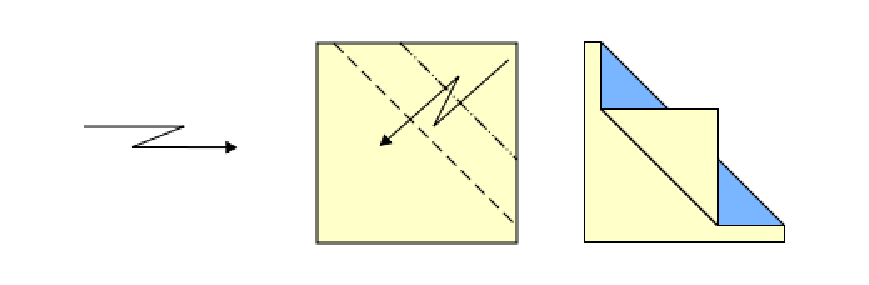
\includegraphics[width=7.5cm]{images/folds_thunderbolt} & \emph{Thunderbolt fold}. A double fold, one of the folds is mountain, the other is valley. An arbitrary angle can be specified for both folds (a different one for each of them).\\
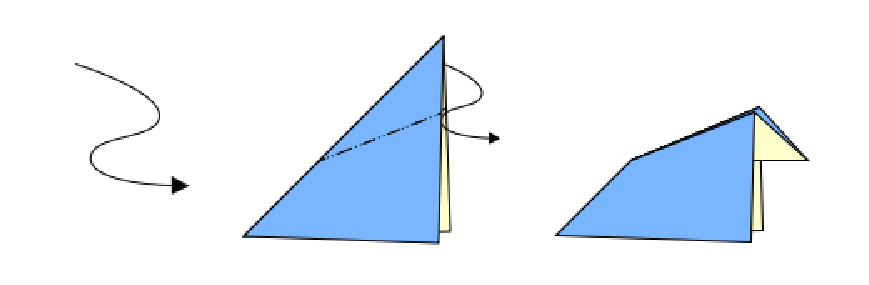
\includegraphics[width=7.5cm]{images/folds_reverse_inside} & \emph{Inside reverse fold}. Tuck a tip of a flap\footnote{A triangle standing out of the paper, which consists of at least two paper layers.} inside. Uses two mountain folds for side creases, and a valley fold for the inner centre line. For every paper configuration, there exists only one angle for the created folds which guarantees to preserve the paper properties.\\
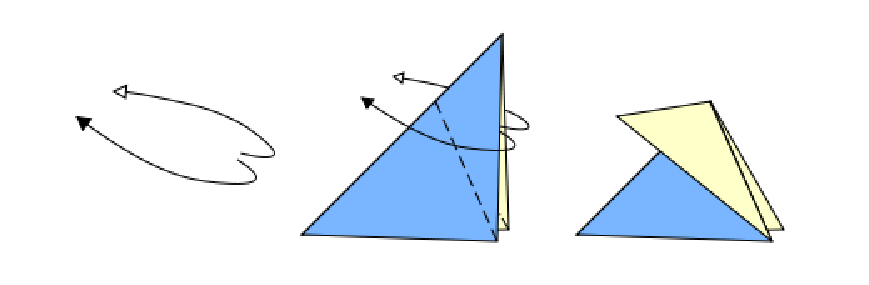
\includegraphics[width=7.5cm]{images/folds_reverse_outside} & \emph{Outside reverse fold}. Wrap a tip of a flap\footnotemark[\value{footnote}] around its outer side. Uses two valley folds for side creases, and a mountain fold for the outer centre line. For every paper configuration, there exists only one angle for the created folds which guarantees to preserve the paper properties.\\
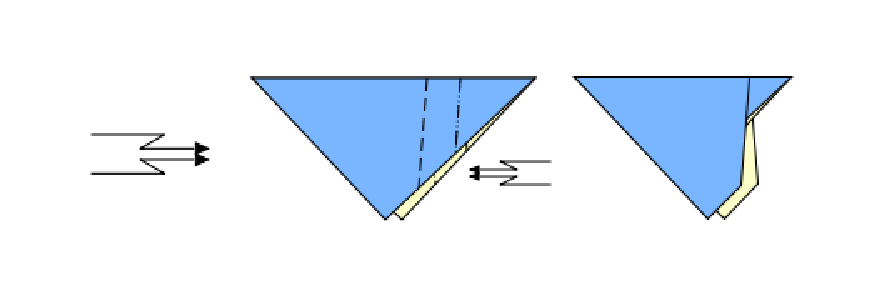
\includegraphics[width=7.5cm]{images/folds_crimp_inside} & \emph{Inside crimp fold}. This is a double fold where both folds are inside reverse folds.\\
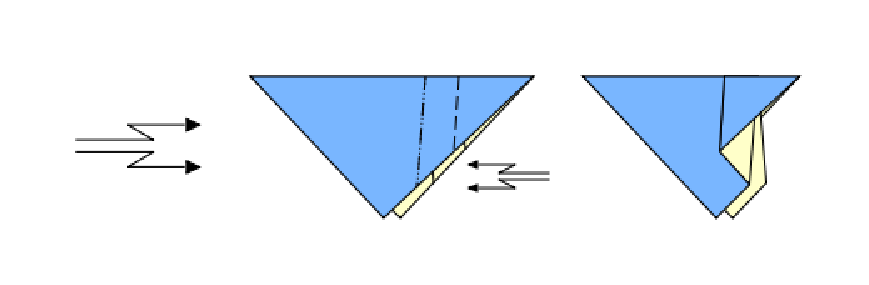
\includegraphics[width=7.5cm]{images/folds_crimp_outside} & \emph{Outside crimp fold}. This is a double fold where both folds are outside reverse folds.\\
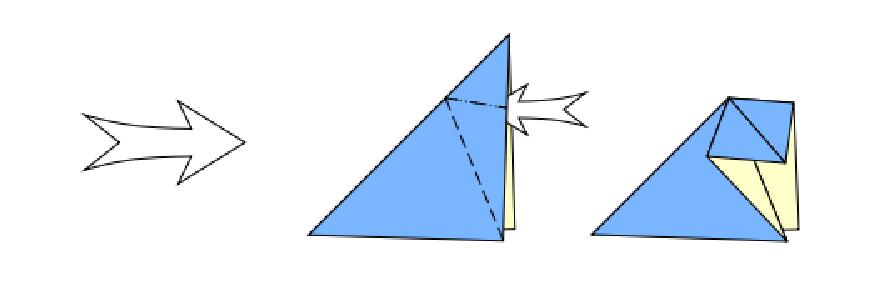
\includegraphics[width=7.5cm]{images/folds_open} & \emph{Open fold}. Open or squash a flap\footnotemark[\value{footnote}] of paper. Origamist doesn't support this operation.\\
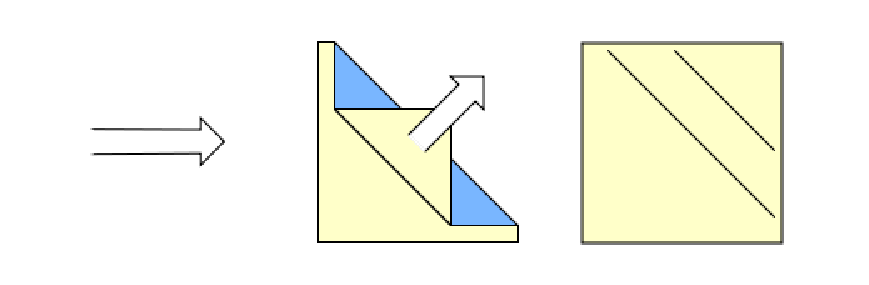
\includegraphics[width=7.5cm]{images/folds_pull} & \emph{Pull fold}. Unfold some previously created folds. Origamist has only partial support for this operation. Only one fold can be unfolded at a time, so eg. atomically unfolding a thunderbolt fold isn't possible.\\
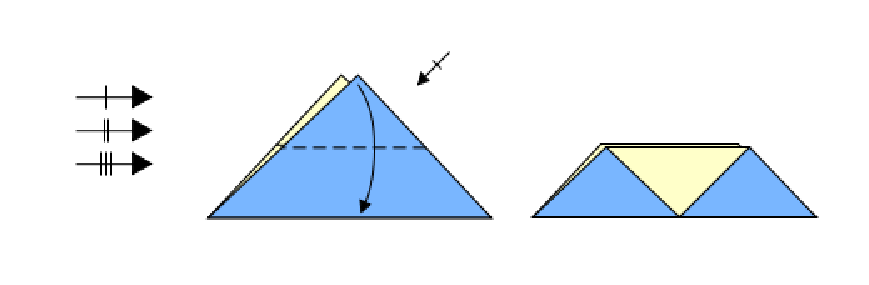
\includegraphics[width=7.5cm]{images/folds_repeat} & \emph{Repeat}. Repeat some previously done operations. This operation hides (for clearness) some steps and substitutes them with the repetition mark.\\
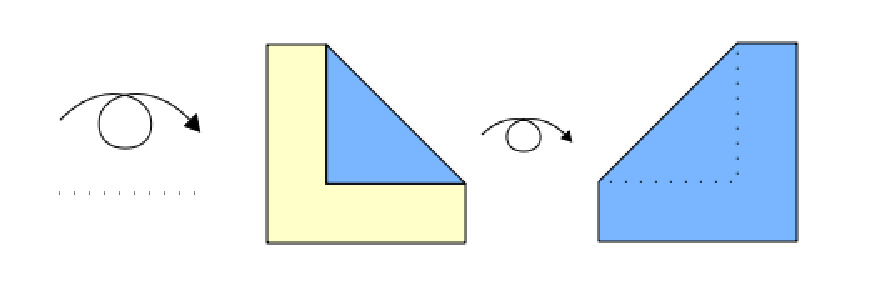
\includegraphics[width=7.5cm]{images/folds_turn_over} & \emph{Turn over}. Turn the paper to the other side. Origamist only supports turning around the horizontal axis of the current view, and a single turning angle - 180 degrees.\\
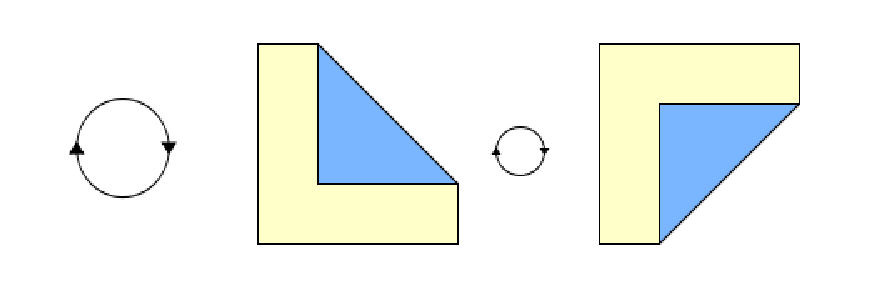
\includegraphics[width=7.5cm]{images/folds_rotate} & \emph{Rotate}. Rotate the model of an arbitrary angle around the current view's direction axis (normal of the screen).\\
\end{longtable}
\end{savenotes}

By using these operations, it is possible to create most of the basic and moderate origami models. Advanced models, however, often require the use of more advanced techniques. Some of them are described in \cite{lang}.

\section{More on operations' marks}
\label{sec:operationMarks}
As can be seen from the above images, some folds are drawn as solid lines, other are drawn as dashed lines and so on. Here are the rules for deciding how to visualise a fold line. The edges of paper are always drawn solid, a little thicker than other lines. Visible creases made in the previous steps (except the current one) are drawn by solid lines (or they can be completely omitted). Invisible\footnote{Folds hidden under other parts of paper. The visualisation using dotted lines is sometimes called X-Ray folds.} folds are drawn by a dotted line (.....). And finally, the creases made in the current step of the manual are drawn as dashed lines (- - - - -) for valley folds and dash-dot lines for mountain folds (-..-..-). Note that the mountain/valley assignment is relative to the side of the paper we look at --- one fold always creates both valley and mountain folds on the opposite sides of paper. The fold with non-convex angle around it is mountain, and the fold with angle less than 180� is valley.

\section{Crease patterns}
\label{sec:creasePatterns}
\emph{Crease patterns}, although they are a very old concept, experience a boom in the latest years as an alternative to classical origami manuals. What is a crease pattern? It is an unfolded origami model, which retains the creases created during the folding process. So, basically, a crease pattern is a set of lines on a straight sheet of paper. Depending on the purpose, the directions of the folds (whether they are mountain or valley) may or may not be specified.

Why are they so popular? This may be due to two wholly different reasons. The first one is that folding a model (with known target shape) from a crease pattern is a challenge, and has no direct instructions. The second reason is that crease patterns are very important in mathematics and computational origami, which is shown in the next chapter.
